\documentclass[11pt, twocolumn]{extarticle}
\usepackage[margin=1.0in]{geometry} 
\usepackage{geometry} 
\geometry{letterpaper}
\usepackage[utf8]{inputenc}
\usepackage[USenglish]{babel}
\usepackage{amsmath,amsfonts,amsthm,graphicx,mathtools,xcolor,parskip, gensymb}
\DeclareMathOperator*{\argmin}{argmin}
\DeclareMathOperator*{\argmax}{argmax}
\usepackage{graphicx}
\usepackage{float}
\usepackage{titling, blindtext, listings, hyperref}
\usepackage[tableposition=above]{caption}
\usepackage{booktabs}
\usepackage{xcolor}
\usepackage{anyfontsize}
\usepackage[font=small]{caption}

% This is not strictly necessary, and may be commented out,
% but it will improve the layout of the manuscript,
% and will typically save some space.
\usepackage{microtype}

%\aclfinalcopy % Uncomment this line for the final submission
%\def\aclpaperid{***} %  Enter the acl Paper ID here

%\setlength\titlebox{5cm}
% You can expand the titlebox if you need extra space
% to show all the authors. Please do not make the titlebox
% smaller than 5cm (the original size); we will check this
% in the camera-ready version and ask you to change it back.

\newcommand\BibTeX{B\textsc{ib}\TeX}
\newcommand{\word}[1]{w_{#1}}
\newcommand{\emb}[1]{\mathbf{w}_{#1}}
\newcommand{\embt}[2]{\mathbf{w}^{(#2)}_{#1}}
\newcommand{\ctx}[1]{\mathbf{c}_{#1}}
\newcommand{\freq}[2]{f^{(#2)}(w_{#1})}

% \setlength{\droptitle}{-4em}%fit in intro on 1 page

\title{
    \Huge NLP Project Description \\ \medskip 
    \large Master IASD - Paris Dauphine - PSL University
}

\author{
    Guillaume Bressan, \
    João Paulo Casagrande Bertoldo, \
    Oskar Rynkiewicz \ 
}

\date{13 February 2020}

% test comment

\raggedbottom

\begin{document}
\maketitle

\section{Overview}

As part of the course \href{https://allauzen.github.io/cours/NLP_IASD/}{\textit{Natural Language Processing}} of the \href{https://www.lamsade.dauphine.fr/wp/iasd/en/}{IASD Master at Paris Dauphine PSL}, we present a description of the project that we will work on. Our project will be based on the paper \textit{Diachronic Word Embeddings Reveal Statistical Laws of Semantic Change} \cite{hamilton-etal-2016-diachronic}. The authors use word embeddings to analyse historical semantic changes in large corpora in different languages. The original project's page with links to all its resources can be found \href{https://nlp.stanford.edu/projects/histwords/data_description.html}{\textit{here}}. Our project will be in \href{https://github.com/joaopcbertoldo/jokar}{\textit{this repository}}.
\par

By training models with sub-corpora of different time periods, the authors were able to use similarity metrics in the embeddings to quantify the rate of meaning changes in the vocabulary over time. They trained three different types of models: PPMI (Positive Point-wise Mutual Information), SVD (Singular Value Decomposition of the PPMI embeddings), and SGNS (Skip-gram with negative sampling, i.e.\@ `word2vec`) \cite{mikolov2013distributed}. Then, the embeddings' axes were aligned using orthogonal Procrustes analysis and tested on several benchmark tasks, resulting in the choice of the SGNS embedding. Finally, they fitted a linear model to quantify the rate of meaning change as a function of word frequency and polysemy.

\section{Data}

The original paper used 6 corpora from Google N-Grams \cite{google-n-grams} and COHA \cite{coha} in 4 languages (English, French, German, and Chinese). For this project, only English will be considered. Of the three datasets in English analysed in the paper, we will consider the COHA corpus. 
\par 

This dataset has been made to be genre-balanced and representative of American English. Two versions of the COHA corpus are available: with and without lemmatization. In the paper, expressive results were obtained for both lemma and raw token levels. For the sake of practicality, we will only use the lemmatized version of the corpus, as it is smaller and "cleaner".
\par

The authors of the original project made available their pre-trained embeddings, as well as historical word frequency, and other metrics used in the paper such as the polysemy score. If possible, we will use these pre-computed metrics to facilitate the comparison between our and their results. A detailed data description can be found \href{https://nlp.stanford.edu/projects/histwords/data_description.html}{\textit{here}}.  
\par

\section{The tasks}

This project will use the original paper's procedure as the starting point and then modify some aspects, that will be specified in the next section. Here, we briefly explain what the initial tasks consist of. 
\par

\subsection*{Obtaining word embeddings \footnote{This corresponds to the section 2 in the paper.}}

Based on 4 benchmark tests, the authors \cite{hamilton-etal-2016-diachronic} concluded that SGNS and SVD strongly outperform PPMI, while the differences between SGNS and SVD are more subtle. For the purpose of discovering word semantic diachronic (historical) changes, SGNS perfomed the best. Therefore, we will consider SGNS model in our project. That being said, SVD outperformed SGNS on the synchronic accuracy task and was most effective for detecting subtle shifts, hence experimentation with other embedding techniques remains an interesting direction.
\par

Each word $\word{i}$ is represented by a low-dimensional vector (its embedding) $\emb{i} \in \mathbb{R}^{d}$  and a context vector $\ctx{i} \in \mathbb{R}^{d}$. These vectors are trained to approximate

\begin{equation}
    \hat{p}\left(w_{j} | w_{i}\right) \propto \exp \left(\mathbf{w}_{i} \cdot \mathbf{c}_{j}\right)
\end{equation}

where $\hat{p}\left(w_{j} | w_{i}\right)$ is the empirical probability of seeing $\word{j}$ in a fixed-length window of text centered on $\word{i}$. The corpus is splitted in chunks of 10 years and a different model is trained for each decade bin. 
\par

As a result, we can extract, for each word and each decade $t$, an embedding $\embt{i}{t}$. However, to be able to compare two embeddings $\embt{i}{t}$ and $\embt{i}{t + 1}$ of the same word, the vector spaces need to have their axes aligned, which is done using orthogonal Procrustes analysis. 
\par

Let $\mathbf{W}^{(t)} \in \mathbb{R}^{d \times|\mathcal{V}|}$\footnote{Here, $\mathcal{V}$ is the set of words (i.e. the vocabulary).} be the matrix of embeddings learned at the decade $t$. The two embeddings are aligned by optimizing:

\begin{equation}
    \mathbf{R}^{(t)}=\argmin _{\mathbf{Q}^{\top} \mathbf{Q}=\mathbf{I}}\left\|\mathbf{Q} \mathbf{W}^{(t)}-\mathbf{W}^{(t+1)}\right\|_{F}
\end{equation}
 
 where $\mathbf{R}^{(t)} \in \mathbb{R}^{d \times d}$ and doing $\mathbf{R}^{(t)} \mathbf{W}^{(t)}$ to adjust the embedding's axes on $t$ to those on $t + 1$. Note that this preserves the cosine similarities between the columns of $\mathbf{W}^{(t)}$.
 
\subsection*{Analysing semantic changes over time \footnote{This corresponds to the section 4 in the paper.}}

The rate of semantic change of $\word{i}$ at $t$ is defined as

\begin{equation}
    \Delta^{(t)}\left(w_{i}\right)=\operatorname{cos-dist}\left(\mathbf{w}_{i}^{(t)}, \mathbf{w}_{i}^{(t+1)}\right)
\end{equation}

Then, we compute \(\tilde{\Delta}^{( t )}(w_{i})\), the normalized log-transformed rate of semantic change  for a word \(w_{i} \in \mathcal{V}\) at time \(t \in \left\{ t_{0},\dots,t_{n} \right\}\). This rate quantifies the semantic displacement \(\tilde{\Delta}^{( t )}(w_i)\) occurring in a pair of consecutive decades, $t$ and $t+1$. 
\par

Finally, they fit a linear model to express \(\tilde{\Delta}^{( t )} ( w_i )\):

\begin{gather*}
\tilde{\Delta}^{( t )} ( w_i ) = \beta_f \log \left( f^{( t )} ( w_i ) \right) +\beta_d \log \left( d^{( t ) } ( w_i ) \right) \\
+ \beta_{t} + z_{w_i} + \epsilon_{w_i}^{( t ) }
\end{gather*} 

which assumes that word's frequency \(f^{( t )} ( w_i )\), polysemy \(d^{( t ) } ( w_i )\), and decade \(t\) impact the semantic change. 

\section{Our project}

At first, we'll fit coefficients \(\beta_f, \beta_d, \beta_t\) using the standard maximum likelihood algorithm, following the authors' approach. We intend to verify that our results will reflect the two statistical laws of semantic evolution discovered by authors: \textit{The law of conformity} and \textit{The law of innovation}.
\par

Next, using their pre-computed embeddings, we will propose a different linear model by including new terms and/or replacing existing ones. For example, we consider initially focusing on the \textit{relative frequency} and "\textit{synonymyty}". The former will consist of transforming the word frequencies such that $\sum^{|\mathcal{V}|}_{i=1} \freq{i}{t} = 1$. The latter would be some metric (to be defined) that measures the "amount of words close enough to $\word{i}$" - as if it captured the "inverse" of the polysemy.
\par

Finally, consider the SGNS architecture as represented in Figure \ref{word2vec-schematic}. We will add a second hidden layer to the model and compare both the shallow and deep embeddings with those of the original paper.

\begin{figure}[H]
    \centering
    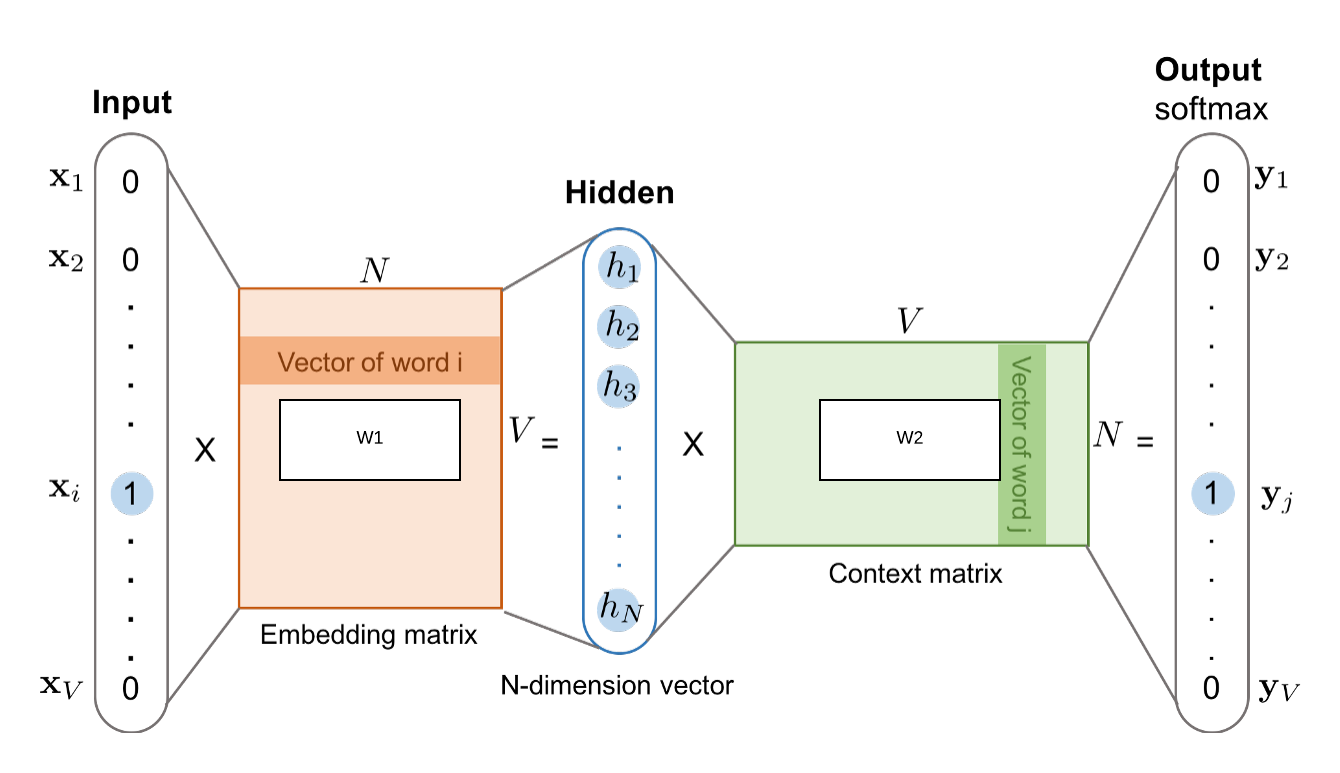
\includegraphics[width=0.45\textwidth]{word2vec.png}
    \caption{
        \label{word2vec-schematic}
        schematic diagram of the Word2Vec model (\href{https://lilianweng.github.io/lil-log/2017/10/15/learning-word-embedding.html}{link to source)}
    }
\end{figure}

For the sake of inspiration, we might try to reproduce some of what other authors have done in similar papers like \cite{dubossarsky-etal-2017-outta},  \cite{dynamic-word-embeddings}, \cite{carlo2019training}, or \cite{delpech2018unsupervised}.

\bibliographystyle{abbrv}
\bibliography{refs}

\end{document}

